\documentclass[conference]{IEEEtran}
\IEEEoverridecommandlockouts
% The preceding line is only needed to identify funding in the first footnote. If that is unneeded, please comment it out.
\usepackage{cite}
\usepackage{amsmath,amssymb,amsfonts}
\usepackage{algorithmic}
\usepackage{graphicx}
\usepackage{textcomp}
\usepackage{xcolor}
\usepackage{tabularx}
\usepackage{multirow}
\usepackage{graphics} % for pdf, bitmapped graphics files
\usepackage{subfig}
\usepackage{subcaption}
\usepackage{hyperref}
\usepackage{academicons}
\usepackage{xcolor}
\usepackage{listings}
\usepackage{tabularx} % Asegúrate de incluir este paquete

\usepackage{tikz}
\usetikzlibrary{shapes.geometric, arrows}

\usetikzlibrary{shapes.geometric, arrows}

\tikzstyle{startstop} = [rectangle, rounded corners, minimum width=3cm, minimum height=1cm,text centered, draw=black, fill=red!30]
\tikzstyle{process} = [rectangle, minimum width=3cm, minimum height=1cm, text centered, draw=black, fill=blue!30]
\tikzstyle{arrow} = [thick,->,>=stealth]


\def\BibTeX{{\rm B\kern-.05em{\sc i\kern-.025em b}\kern-.08em
		T\kern-.1667em\lower.7ex\hbox{E}\kern-.125emX}}

% Color Enlace
\definecolor{colorEnlace}{RGB}{0, 0, 0}
\hypersetup{
	colorlinks=true,
	linkcolor=colorEnlace,
	citecolor=colorEnlace,
	urlcolor=colorEnlace,
	pdfauthor={Davis Bremdow Salazar Roa},
	pdftitle={Instrumentación Electrónica - ECG}
}
\definecolor{mybg}{rgb}{0.97,0.97,0.97}
\definecolor{mygray}{gray}{0.4}
\definecolor{mygreen}{rgb}{0,0.6,0}
\definecolor{myblue}{rgb}{0,0,0.8}
\definecolor{mypurple}{rgb}{0.58,0,0.82}
\definecolor{myred}{rgb}{0.7,0,0}

\lstdefinelanguage{MatlabEnhanced}{
	language=Matlab,
	morekeywords={[2]linspace,plot,title,xlabel,ylabel,legend,grid},
	morekeywords={[3]sin,cos,exp,log,sqrt},
	keywordstyle=\color{myblue}\bfseries,
	keywordstyle=[2]\color{mypurple},
	keywordstyle=[3]\color{myred},
	commentstyle=\color{mygreen}\itshape,
	stringstyle=\color{mygray},
	morecomment=[l]%
}

\lstset{
	language=MatlabEnhanced,
	backgroundcolor=\color{mybg},
	frame=single,
	basicstyle=\ttfamily\small,
	showstringspaces=false,
	numbers=none,              %
	xleftmargin=0pt,           %
	framexleftmargin=0pt,      
	framexrightmargin=0pt,
	framextopmargin=2pt,
	framexbottommargin=2pt,
	breaklines=true,
	tabsize=1,
}

% Control 
\usepackage{amsmath}
\begin{document}
	
	\title{Acondicionamiento de señal para la obtención de electrocardiogramas}
	\author{
		\makebox[\textwidth][c]{\large\textbf{Universidad Nacional de San Antonio Abad del Cusco}}\\
		\makebox[\textwidth][c]{\normalsize\textit{Escuela profesional de Ingeniería Electrónica}}\\
		\makebox[\textwidth][c]{\normalsize\textit{Asignatura: Instrumentación Electrónica}}\\
		\and
		\IEEEauthorblockN{Ing. Alex Jhon Quispe Mescco}
		\IEEEauthorblockA{Ingeniero Electrónico \\
			Cusco, Perú \\
			alex.quispe@unsaac.edu.pe}
		\and
		\IEEEauthorblockN{Davis Bremdow Salazar Roa - 200353}
		\IEEEauthorblockA{Estudiante de Ingeniería Electrónica \\
			Cusco, Perú \\
			200353@unsaac.edu.pe}
	}
	
	\maketitle
	\begin{abstract}
	Una área dentro de la biomedicia y de vital importancia es la obtención de electrocardiogramas que permiten a los especialistas del área de la salud detectar anomalías relacionadas al corazón para brindar un tratamiento o recomendaciones para el cuidado del paciente, por lo que es de vital importancia que representación sea lo más fiel al origen, siendo así que se presenta el estudio y aplicación de los CI de vanguardia para el objetivo de este propósito y para el cual se emplea un diseño que integra diferentes etapas de facilitan la obtención de tal señal hasta su procesamiento en un microcontrolador.
	\end{abstract}
	
	\begin{IEEEkeywords}
		Amplificadores de Instrumentación, CMRR, Electrocardiograma, Aplicaciones Biomedicas 
	\end{IEEEkeywords}
	
%	Contenido del documento
	\section{Introducción}
	
	La instrumentación es el proceso mediante el cual una señal de diferentes características se adecúa según su tipo para expresarla en niveles normalizados de corriente o voltaje, empleando para ello diferentes etapas según las necesidades de las mismas.
	
	Para la instrumentación y obtención de un electrocardiograma en primera instancia se debe considerar, los puntos de medición en el cuerpo y humano y los respectivos potenciales de referencia, los electrodos como elementos de sensado, la etapa de instrumentación para la supresión de ruido, el filtrado para eliminar componentes indeseadas en frecuencia y finalmente en caso de ser necesario el uso de ADC para el tratamiento digital de la información.
	
	Aunque cada parte es de vital importancia para la obtención del electrocardiograma en el presente informe se tendrá como elemento principal de estudio los \textbf{Circuitos Integrados de Instrumentación} que desde su desarrollo en 1950 hasta la fecha se cuenta con una gran variedad que los puede clasificar por su especificidad para su empleo en ciertas áreas involucrando dentro de ello la electrónica.
	
	En la actualidad el desarrollo de amplificadores de instrumentación toma como referencia el empleo de integrados de instrumentación ampliamente utilizados como lo son el INA128, AD20 o el AD627 como punto de partida, agregando nuevos bloques externos para agregar más funcionalidad, generando la siguiente generación de circuitos integrados de instrumentación.
	
	\section{Marco Teórico}
	
	Para facilitar la compresión de los todos los procesos fenómenos físicos y biológicos involucrados en la obtención de un electrocardiograma es necesario definir algunos conceptos base que se mostraran en las siguientes sub secciones del informe
	
	\subsection{Amplificador de Instrumentación}
	Circuito electrónico de precisión en configuración diferencial, empaquetado de forma monolítica (Circuito Integrado) y de ganancia configurable mediante el empleo de una resistencia $R_{gain}$ externa.
	
	En la figura \ref{fig:amplificador-instrumentacion} se muestra la configuración más básica para un amplificador de instrumentación.
	\begin{figure}[h]
		\centering
		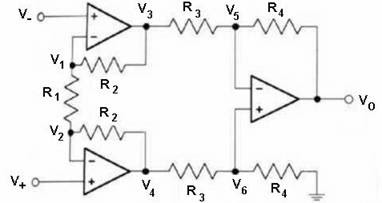
\includegraphics[width=0.5\textwidth]{media/amplificador-instrumentacion}
		\caption{Amplificador de Instrumentación - Configuración inicial/básica}
		\label{fig:amplificador-instrumentacion}
	\end{figure}
	
	\subsection{Ruido}
	
	Perturbación indeseada localizada en todo el espectro electromagnético de diferente origen de naturaleza constructiva y/o aditiva, siendo la más perjudicial para el actual proceso la generada por los aparatos electrónicos.
	
	\subsection{Biopotencial}
	El cuerpo humano se encuentra conformado por una gran cantidad de Iones y cuyas cantidades están expresadas en forma de concentración en el interior y exterior de la membrana celular o capa que separa ambas cantidades, en este proceso mediante la ganancia y perdida de electrones debido a procesos químicos, son creados los biopotencial que generan un campo eléctrico que a su vez genera un campo eléctrico respecto a la distancia propagándose en todas las direcciones.
	
	El acto de medir el cambio de este potencia debido a los procesos bioquimicos producidos en el cuerpo es lo que nos permite generar los electrocardiogramas que nos brinda información acerca del funcionamiento del corazón.
	
	\subsection{Electrodos}
	Es un conductor que permite vincular un elemento no metálico con un circuito eléctrico el cual es usado ampliamente en aplicaciones químicas y biomedicas, siendo el último caso el de interés para el informe realizado, en la figura \ref{fig:electrodo} se muestra un esquema gráfico del electrodo.
	
	\begin{figure}[h]
		\centering
		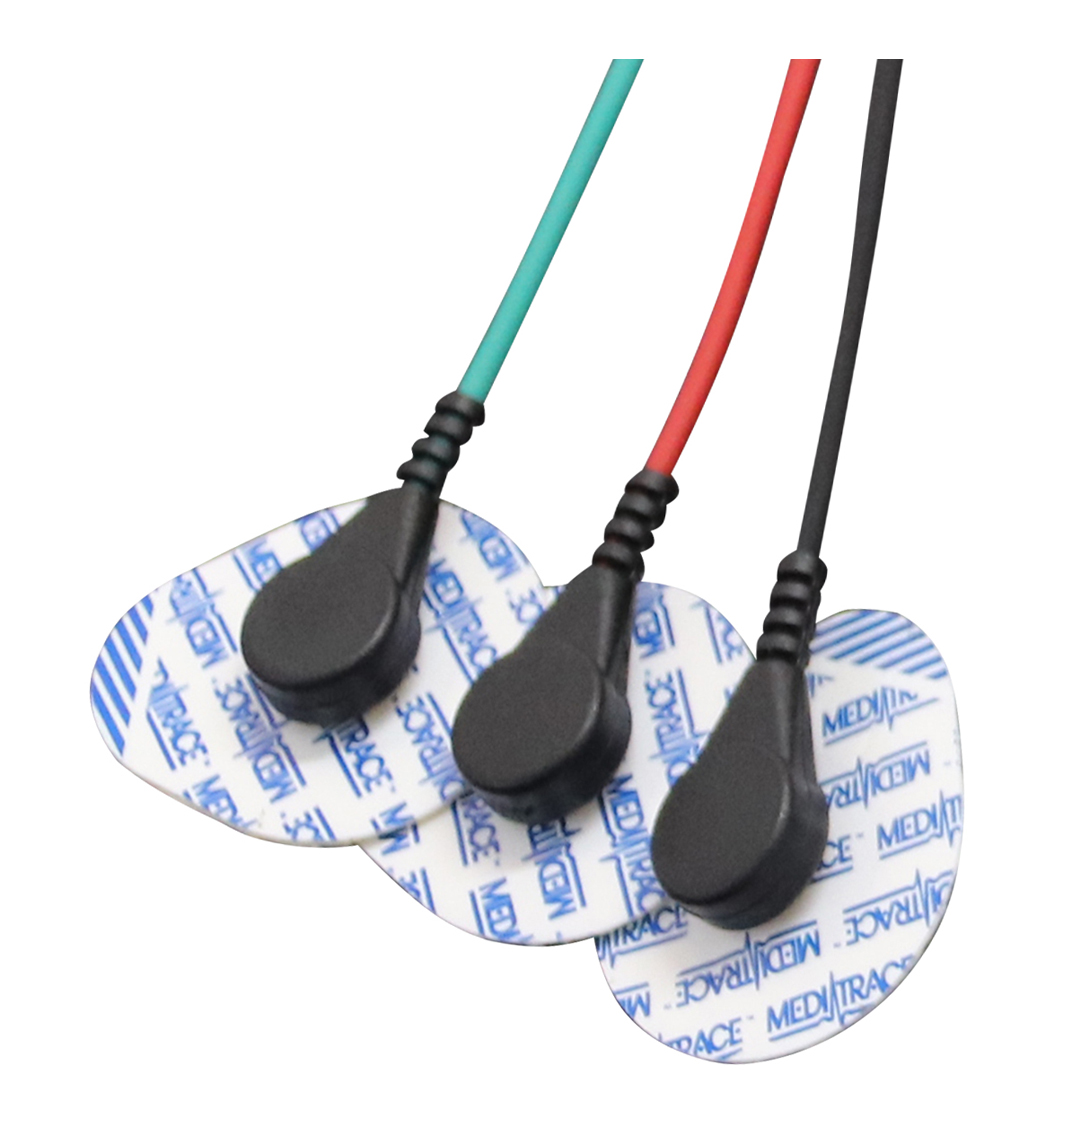
\includegraphics[width=0.4\textwidth]{media/electrodo}
		\caption{Electrodo}
		\label{fig:electrodo}
	\end{figure}
	
	\section{Vectores de potencial en el cuerpo}
	
	Además de una magnitud el voltaje debido al campo eléctrico generado en el cuerpo humano este se representa en forma de vector los cuales por su naturaleza nos índica el dirección del potencial eléctrico, esta representación se puede apreciar en la figura \ref{fig:vectores-potencial}.
	
	\begin{figure}[h]
		\centering
		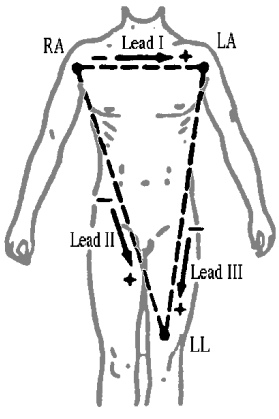
\includegraphics[width=0.4\textwidth]{media/vectores-potencial}
		\caption{Vectores de potencial - Puntos de referencia para la medición de una ECG}
		\label{fig:vectores-potencial}
	\end{figure}
	
	En el esquema se puede apreciar 3 puntos de potencial, uno ubicado en el brazo derecho (RA), el siguiente el brazo izquierdo (LA) y el punto final en la pierna izquierda (LL) que es el punto de referencia o tierra.
	
	\section{Amplificador de Instrumentación}
	
	Una vez definidos los parámetros de medición, así como los lugares de referencia para ello, se paso a realizar el estudio del amplificador de instrumentación a emplear teniendo en cuenta para ello el estado del arte actual sobre esta tecnología.
	
	Como se puede apreciar en \cite{9455865} se propone la creación de un amplificador de instrumentación (IA) - CBIA de 2,24 NEF (Noise Effiency Factor) con tecnología de 180nm para el seguimiento de señales ECG mediante el empleo de 2 etapas una de transconductancia y otra de transimpedancia para lograr un alto SNR o reducción del ruido.
	
	Por otro lado en \cite{10101028} publicado en 2023, se describe el prototipo de un amplificador de instrumentación de bajo costo y buen rendimiento en función a los C -  amplificadores operacionales LM324/LM741 agregando una etapa de salida mediante IoT para su monitoreo a distancia. Así mismo en el mismo año en \cite{10373502} se propone la creación de un amplificador de instrumentación (INA) basado en tecnología CMOS de 90nm con una alimentación de 1.2v (bajo consumo) para aplicaciones biomedicas en donde se tiene una mayor susceptibilidad al ruido, garantizando un alto rendimiento con un CMRR de 98.25dB.
	
	En el estado del arte además se puede destacar el empleo de diferente técnicas que en lugar de proponer una nueva topologia de componentes para la implementación de un IA, guardan un enfoque estructural añadiendo nuevos etapas al CI de instrumentación ya existente, agregando capacidades o mejorando su respuesta frente al ruido.
	
	Finalmente para el acondicionamiento y obtención del electrocardiograma se tuvo como referencia \cite{pantuprecharat2023ecg} en la cual se describe la implementación de un amplificador frontal de instrumentación para ECG, utilizando para tal propósito transportadores de corriente (CCII) de segunda generación y un amplificador de instrumentación (CBIA) para la reducción de ruido en la entrada logrando un CMRR de 53dB que incluye dentro de su arquitectura un filtro pasa baja para la obtención de señales deseadas y limitante de ruido, así como amplificador de ganancia variable (VGA) para finalmente integrar un ADC para el tratamiento de la señal de forma digital.
	
	El esquema genera propuesto se muestra en la figura \ref{fig:ecg-amplifier} en la cual se describe la entrada, el bloque de amplificador de instrumentación, el filtro pasabajos, el amplificador de ganancia variable y finalmente la etapa analógica digital.
	
	\begin{figure}[h]
		\centering
		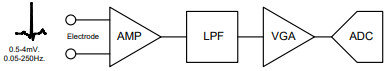
\includegraphics[width=0.5\textwidth]{media/ecg-amplifier}
		\caption{Diagrama de bloques - Amplificador de Instrumentación ECG}
		\label{fig:ecg-amplifier}
	\end{figure}
	
	Un esquema detallado del transportador de corriente (CCII), el amplificador de instrumentación y el circuito equivalente de unir ambas etapas (front-end), se muestra en las figuras \ref{fig:transportador-corriente}, \ref{fig:ia-propuesto}, \ref{fig:circuito-equivalente} respectivamente.
		
	\begin{figure}[h]
		\centering
		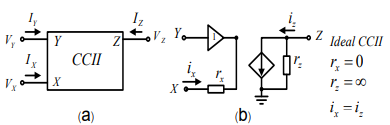
\includegraphics[width=0.4\textwidth]{media/transportador-corriente}
		\caption{Modelo del transportador de corriente (CCII)}
		\label{fig:transportador-corriente}
	\end{figure}
	
	\begin{figure}[h]
		\centering
		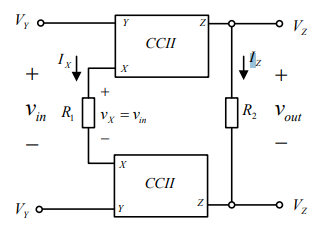
\includegraphics[width=0.4\textwidth]{media/ia-propuesto}
		\caption{Esquema de amplificador de instrumentación}
		\label{fig:ia-propuesto}
	\end{figure}
	
	\begin{figure}[h]
		\centering
		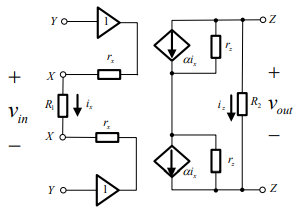
\includegraphics[width=0.4\textwidth]{media/circuito-equivalente}
		\caption{Circuito equivalente resultante - Front-end}
		\label{fig:circuito-equivalente}
	\end{figure}
	
	Los resultados de ganancia de los esquemas circuitales se definen como la relación de 2 resistencias multiplicadas por el factor de $\alpha$ propio del amplificador de ganancia controlada, obteniendo la relación \ref{eq:ganancia-ia}.
	
	\begin{equation}
		\frac{V_{out}}{V_{in}} = \alpha\frac{R_2}{R_1}
		\label{eq:ganancia-ia}
	\end{equation}
	
	Donde $R_2$ y $R_1$ son resistencias externas y factor $\alpha$ se considera idealmente 1, obteniendo así que la ganancia total del circuito integrado depende enteramente de la relación de resistencias.
	
	\section{Empleo de CI para la medición de una ECG}
	
	Para la obtención de una ECG mediante el circuito propuesto en \cite{pantuprecharat2023ecg} cada etapa desde la ubicación de los electrodos hasta la salida en un microcontrolador se representaran mediante bloques funcionales que se muestran en la figura \ref{fig:esquema-conexion-uso}.
	
	\begin{figure}[h]
		\centering
		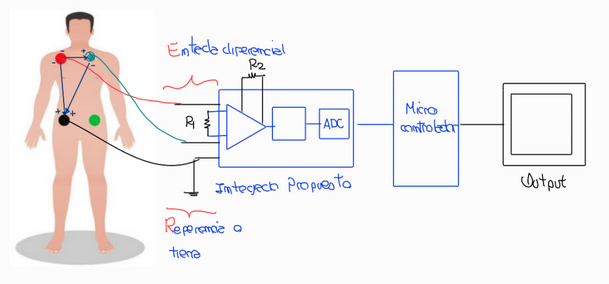
\includegraphics[width=0.5\textwidth]{media/esquema-conexion-uso}
		\caption{Esquema de conexión - Uso del CI para ECG}
		\label{fig:esquema-conexion-uso}
	\end{figure}
	
	Y en el cual para modificar la ganancia de salida del circuito tan solo es necesario modificar las ganancias $R_1$ y $R_2$ según lo requerido, teniendo en cuenta que el voltaje de salida estándar para un electrocardiograma es de 1mv o 2mv, pudiendo extender esto hasta los niveles deseados para su visualización en un monitor.
	
	Además se debe considerar que la salida del ADC implementado tiene una salida serial para su conexión al microcontrolador siendo así que la cantidad de bits para la conversión no se especifican de forma explicita, sin embargo se asume un cantidad mínima de 9 bits para obtener una resolución adecuada para conversión con un voltaje de entrada de 1mV.

	
	\bibliographystyle{IEEEtran}
	\bibliography{biblio}
\end{document}
